%!TEX root = ../BoYu-Dissertation.tex
\graphicspath{{Figures/}}
\chapter{Understanding Awareness} % (fold)
\label{cha:understanding_awareness}

\fxfatal{Add a general diagram to layout the framework, discuss existing work in the framework, add a table to compare and summarize the literature}

The concept of awareness has come to play a central role in both social and technical research in CSCW. However, what in CSCW labeled as `awareness' has little in common, besides the fact that it represents some aspect of human interaction that is important for successful collaboration \cite{schmidt2002a}. In a broad sense, two types of awareness can be distinguished in the CSCW research area: \emph{social awareness} and \emph{task-oriented awareness} \cite{prinz1999a,schmidt2002a}.

\emph{Social awareness} addresses the availability of different kinds of information about the social context of the team members, e.g. awareness about what they are doing, if they are talking to someone, if they can be disturbed etc. \emph{Social awareness} thus is conceived of as something that engenders ``informal serendipitous interactions'' \cite{hudson1996a} and ``a shared space for community building'' \cite{Dourish1992}. Awareness of the general social context is an important aspect of collaborative work, especially in domains where the the actors are engaged in cooperative work in a loose and broad sense, or domains where socialization is crucial \cite{schmidt2002a}.

However, when the tasks of collaborating actors become closely interdependent on each other, more urgent concerns need to be given to the aspect of \emph{task-oriented awareness}. The \emph{task-oriented awareness} focuses on practices through which actors seamlessly align and integrate their distributed and yet interdependent activities, e.g. awareness of things being done or in need of being done, of developments within the joint effort that may be advantageous or detrimental for one’s own work, of occurrence that makes one’s work more urgent or leads to changes to the intended course of actions, etc. \cite{schmidt2002a}. The major difference of \emph{task-oriented awareness} from \emph{social awareness} is that it focuses on activities performed to achieve a specific shared goal \cite{carroll2003a} and the actor’s being interdependent in their work \cite{schmidt2002a}, which lead to the unavoidable requirement for coordination.

In this study, we focuses on the \textbf{task-oriented aspect of awareness}, because the primary goal of supporting awareness in this study is motivated by the actors' being interdependent in their work and hence by the unavoidable requirements of coordinating and integrating their various actions in distributed geo-collaborative activities.

Within the scientific investigation into task-oriented awareness phenomena in collaboration, two lines of research can be identified. On one hand is the research aiming to establish conceptual understanding of the awareness phenomena from the cognitive and social aspects \cite{Salmon2008}, and on the other hand is an increasing bearing on system design and development in particular technologies to promote awareness \cite{rittenbruch2009a}. Although our work has an emphasis on the second aspect, i.e. the supportive technologies to promote awareness, we believe that a solid conceptualization of awareness phenomena in collaboration is extremely important for awareness promotion. System designers need to know what awareness might comprise and also how it is built and maintained in order to identify the specific awareness features they want to support \cite{Stanton2006}. 

As a result, before we move to the computational issues for awareness promotion, this chapter attempts to identify which of the existing theories and conceptualization of awareness in the literature is the most suitable for understanding the awareness phenomena in real world complex collaborative activities. A review and critique of what is currently known on the concept of awareness at both individual and team levels is presented, following which an integrated conceptual framework of awareness phenomena in complex collaborative activities is presented. In next chapter, we will show how such a conceptual framework helps us to evaluate existing computational awareness models and systems, and informs our design of the computational framework for awareness promotion.

\section{Situation Awareness}
\label{sec:awareness_in_individuals}
Research into awareness at the individual level originated from the study of situation awareness (SA) in the human factors research community. Situation awareness is considered as knowledge created through interaction between a person and his/her environment, i.e. ``knowing what is going on'' in the situation \cite{Endsley1995}. A good general definition of situation awareness is as ``the up-to-the minute cognizance required to operate or maintain a system'' \cite{Adams1995}. Although most of the situation awareness models in the literature are individual focused theories \cite{Salmon2008}, it has also been well recognized as an important element in collaborative environments. For example, Gutwin and Greeenberg \cite{Gutwin2002} view their workspace awareness as a specialization of situation awareness tied to the specific setting of the shared workspace. The concept of activity awareness proposed by Carroll et al. also subsumes situation awareness with an emphasis on aspects of the situation that have consequences for group work towards shared goals \cite{carroll2003a}. Hence, to understand the awareness phenomena in collaboration, it is important to start with understanding the practice of how individuals maintain and develop the situation awareness.

The human factors community has not settled on a common explanation of situation awareness, but we still can summarize some of the important characteristics that are well recognized in the literature, and also applicable to collaborative environments:

\begin{enumerate}
	\item The products of awareness is the knowledge about the elements of the environment that is hierarchically structured \cite{Endsley1995}.
	\item The awareness phenomena should be seen as both product and process. As product, it is the knowledge that an actor can make use of. As process, it includes the cognitive processes through which the knowledge is achieved and developed) \cite{Adams1995}.
	\item The process of achieving and developing awareness revolves around internally held, mental models, which contain activated information regarding current situations \cite{Smith1995}. The activation of awareness information into the mental models are directed by the actor's activity \cite{Bedny1999}.
\end{enumerate}

We elaborate these three characteristics in the following of this section.

\subsection{Hierarchically Structured Awareness Knowledge} % (fold)
\label{sub:awareness_as_product}
Among the numerous attempts at specifying the products of situation awareness, i.e. what must be known to solve a class of problems posed when interacting with a dynamic environment \cite{Salmon2008}, Endsley's three-level model \cite{Endsley1995} has undoubtedly received the most attention. The three-level model describes situation awareness as the operator's internal model of the state of the environment, comprising three hierarchical levels that is separate to the process used to achieve it \cite{Smith1995}:

\begin{enumerate}
	\item Level 1: \emph{perception of relevant elements in the environment}. An actor must first be able gather perceptual information in the surrounding environment, and be able to selectively attend to those elements that are most relevant for the task at hand. At this stage, the information is merely perceived and no further processing takes place. 
	\item Level 2: \emph{Comprehension of task-related elements in Level 1}. Level 2 involves the interpretation of the perceptual information from Level 1 in a way that allows an actor to comprehend or understand its relevance in relation to their tasks and goals.
	\item Level 3: \emph{Projection of the states in the near future}. Using a combination of Level 1 and Level 2 awareness-related knowledge and experience in the form of mental models, actors forecast likely future states in the situation.
\end{enumerate}

Endsley's three-level model presents an intuitive description of situation awareness and has been applied in a plethora of different domains \cite{Wickens2008}. Its simplicity and the division of SA into three hierarchical levels allows the construct to be measured easily and effectively \cite{endsley1995measurement}, and also supports the abstraction of situation awareness requirements and the development of design guidelines \cite{Salmon2008}. Furthermore, it has been extended in order to describe team situation awareness \cite{endsley2001model}, and the three levels of awareness information are applicable in many collaborative situations \cite{Gutwin2002}.

Despite its popularity, the three-level mode has some important flaws. One of the key assumptions of the three-level model is the separation between depicting situation awareness as a product and the cognitive processes used to achieve it \cite{Salmon2008}, which leads to the inability to cope with the dynamic nature of situation awareness \cite{Smith1995}. For example, Uhlarik and Comerford \cite{uhlarik2002review} suggest that the process of achieving situation awareness presented by the three-level model is both static and finite. Nevertheless, the model is also criticized by the ill-defined concept of mental models. Although Endsley's model emphasizes the critical roles of mental models in directing attention to critical elements in the environment (Level 1), integrating the elements to aid understanding of their meanings (Level 2), and generating possible future states (Level 3), the definition only includes the long-term knowledge that is formed by training and experiences, more important factors, such as the actor's goals, conceptual model of the current situation, are neglected \cite{Bedny1999}.
% subsection awareness_as_product (end)

\subsection{The Development of Awareness} % (fold)
\label{sub:awareness_as_process}
To address the dynamic nature of situation awareness, many researchers have used Niesser's perceptual cycle model \cite{neisser1976cognition} to clarify the cognitive components involved in the acquisition and development of situation awareness \cite{Smith1995,Adams1995,Gutwin2002,Stanton2009}. According to the perceptual cycle model (Figure. \ref{fig:perceptual_cycle}), an actor's interaction with the world continues in an infinite cyclical nature. By perceiving the available information in the environment, the actor modifies its knowledge. Knowledge directs the agent's activity in the environment. That activity samples and perhaps anticipates or alters the environment, which in turn informs the agent. The informed, directed sampling and/or anticipation capture the essence of behavior characteristic of situation awareness.

\begin{figure}[htbp] %  figure placement: here, top, bottom, or page
   \centering
   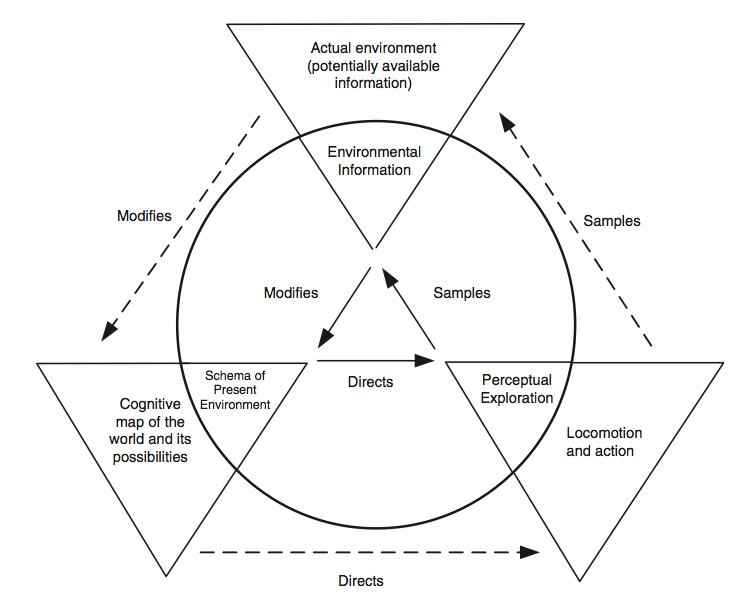
\includegraphics[width=5in]{perceptual_cycle.jpg} 
   \caption{Niesser's Perceptual Cycle Model \cite{Salmon2008}}
   \label{fig:perceptual_cycle}
\end{figure}

Based upon Niesser’s perceptual cycle model, Smith and Hancock suggest that situation awareness is neither resident in the world nor in the person, but resides through the interaction of the person with the world \cite{Smith1995}. Thus they viewing situation awareness as a generative process in `an adaptive cycle of knowledge, action and information' \cite{Smith1995}. In a similar fashion, Adams et al. \cite{Adams1995} used a modified version of Niesser’s perceptual cycle model to describe how situation awareness works. They argue that the process of achieving and maintaining situation awareness revolves around internally held mental models, which facilitate the anticipation of situational events, directing an actor's attention to cues in the environment and directing their eventual course of action. An actor then conducts checks to confirm that the evolving situation conforms to their expectations. Any unexpected events serve to prompt further search and explanation, which in turn modifies the actor's existing model. Gutwin and Greeenberg used the perception-action cycle to explain how the awareness is maintained in a shared workspace, in which awareness knowledge both directs and is updated by perceptual exploration of the workspace environment \cite{Gutwin2002}.

Unlike the three-level model that depicts SA as a product separate from the processes used to achieve it, models based on the perceptual cycle view situation awareness as both process and product, offering an explanation of the cognitive activity involved in the development of situation awareness, and also a judgment as to what the product of SA comprises \cite{Salmon2008}. One of the key assumptions of these models is the interplay between the awareness information and the internal mental model of current situation. In the process of awareness development, some knowledge is activated and integrated into the mental model, while some becomes inactive or removed from the mental model. Although Smith and Hancock suggested that the adaptation of awareness information into the mental model should be goal-directed, i.e. it must reside in the task environment rather than in the actor's head \cite{Smith1995}, little detail has been given about the cognitive processes that guide the selection and interpretation of awareness information into the mental models.
% subsection awareness_as_process (end)

\subsection{Activity Directed Awareness Process} % (fold)
\label{sub:activity_directed_awareness_process}
Bedny and Meister propose a description of situation awareness based on the activity theory in an attempt to clarify the cognitive processes involved in the interpretation of awareness information \cite{Bedny1999}. Based on the activity theory, they purport that individuals possess goals that represent an ideal image or desired end state of activity, which direct them towards the end state or methods of activity (or actions) that permit the achievement of these goals. It is the difference between the goals and the current situation that motivates an individual to engage in the awareness process and take action towards achieving the goal. They conceptualize activity in three stages: the orientational stage, the executive stage, and the evaluative stage. The orientational stage involves the development of an internal representation or picture of the world or current situation. The executive stage involves proceeding towards a desired goal via decision-making and action execution. Finally, the evaluative stage involves assessing the situation via information feedback, which in turn influences the executive and orientational components.

Instead of considering the actor's internal mental model as a whole, they suggest that the mental model is comprised of several functional blocks as presented in Figure \ref{fig:activity_sa}. Each functional block has a specific role to play in the development and maintenance of situation awareness and that the blocks orientate themselves towards the achievement of situation awareness. The interpretation of incoming information (function block 1) is influenced by an individual’s goals (function block 2), conceptual model of the current situation (function block 8), and past experience (function block 7). This interpretation then modifies an individual’s goals and experience and conceptual model of the current situation. Critical environmental features are then identified (function block 3) based upon their significance to the task goals and the individual’s motivation towards the task goal (function block 4), which directs their interaction with the world (function block 5). The extent to which the individual proceeds to engage the task goals is determined by their goals (function block 2) and their evaluation of the current situation (function block 6). The resultant experience derived from the individual’s interaction with the world is stored as experience (function block 7), which in turn informs their conceptual model (function block 8).

\begin{figure}[htbp] %  figure placement: here, top, bottom, or page
   \centering
   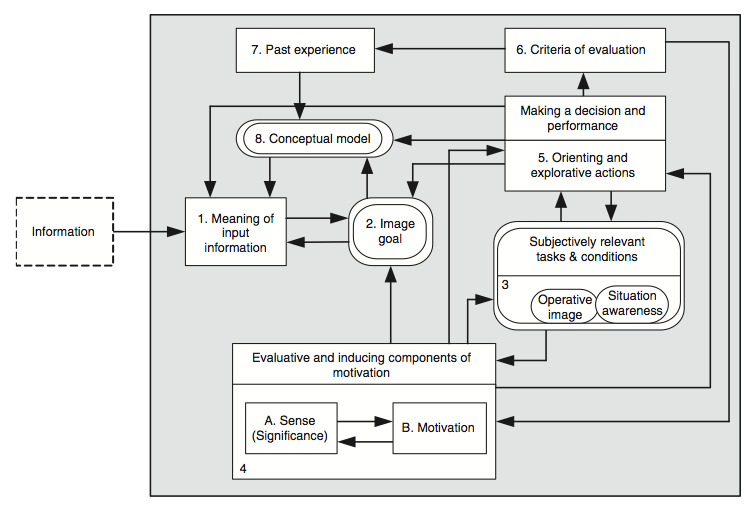
\includegraphics[width=5.5in]{activity_sa.jpg} 
   \caption{Bedny and Meister's Activity-Directed Awareness Process \cite{Bedny1999}}
   \label{fig:activity_sa}
\end{figure}

Based on the activity theory, Bedny and Meister clearly elucidate the functional blocks within the actor's mental model and their roles in the development of situation awareness \cite{Bedny1999}. Their model clearly shows how the actor's goals and activities play a central role to drive the process of awareness development. However, like most other situation awareness-related models, Bedny and Meister's activity theory model does not attempt to cater for, or explain the awareness phenomena in collaborative settings.
% subsection activity_directed_awareness_process (end)

\section{Awareness In Collaboration} % (fold)
\label{sec:awareness_in_collaboration}
The awareness phenomena in collaborative environments is indubitably more complex than situation awareness at the individual level. Salas et al. \cite{salas1995situation} point out that there is a lot more to team level awareness than merely combining individual team member's situation awareness. Beyond knowing what is going on in the environment, in their tasks, team members also need to develop an understanding of the activities of others, which provides a context of their own activities. This context is used to ensure that individual contributions are relevant to the group's shared goal as a whole \cite{dourish1992awareness}. This section reviews three prominent conceptualizations of awareness in collaboration that informs this study: team situation awareness, activity awareness, and distributed team awareness.

\subsection{Team Situation Awareness} % (fold)
\label{sub:team_situation_awareness}
The research on team situation awareness (TSA) attempts to extend the theories and models of situation awareness to collaborative settings. Endsley et al. \cite{endsley2001model} suggest that, during team activities, situation awareness can overlap between team members, in that individuals need to perceive, comprehend and project awareness elements that are specifically related to their specific role in the team, but also elements that are required by themselves and by members of the team. Successful team performance therefore requires that individual team members have good situation awareness on their specific elements and also the same awareness for those elements that are shared. It is therefore argued that, at a simple level, team situation awareness comprises three separate but related components: individual team member's situation awareness; situation awareness of other team members; and situation awareness of the overall team (Figure \ref{fig:tsa}). 

\begin{figure}[htbp] %  figure placement: here, top, bottom, or page
   \centering
   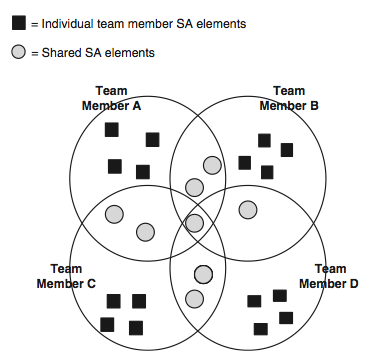
\includegraphics[width=3.5in]{TSA.jpg} 
   \caption{Team Situation Awareness (adapted from Endsley 1995 \cite{Endsley1995})}
   \label{fig:tsa}
\end{figure}

Similar to individual situation awareness, team situation awareness should be considered as a dynamic process. Salas et al. \cite{salas1995situation} propose a framework of team situation awareness that comprises two critical processes, individual situation awareness and team processes. According to them, team situation awareness depends on communications at various levels. The perception of SA elements is influenced by the communication of mission objectives, individual tasks and roles, team capability and other team performance factors. The comprehension of awareness information (i.e. Level 2) is impacted by the interpretations made by other team members, so it is evident that SA leads to SA and also modifies SA, in that individual SA is developed and then shared with other team members, which then develops and modifies team member SA. Thus, a cyclical nature of developing individual SA, sharing SA with other team members and then modifying SA based on other team members’ SA is apparent. 

Most attempts to understand team SA have centered on a `shared understanding' of the same situation. Nofi \cite{nofi2000defining}, for example, defines team SA as: `a shared awareness of a particular situation' and Perla et al. \cite{perla2000gaming} suggest that `when used in the sense of ``shared awareness of a situation'', shared SA implies that we all understand a given situation in the same way'. Shu and Furuta sugggested that TSA comprises both individual SA and mutual awareness and can be defined as `two or more individuals share the common environment, up-to-moment understanding of situation of the environment, and another person's interaction with the cooperative task' \cite{shu2005inference}.

Team situation awareness has been broadly recognized as a critical factor to understand awareness in collaborative environment, because its compatibility to individual situation awareness, and the abstraction of individual awareness process from team processes \cite{shu2005inference,Salmon2008}. However, TSA also has many limitations.

\begin{enumerate}
 	\item First, a critical factor of team situation awareness is to define the configuration of shared situation awareness requirements, i.e. the degree to which team members understand which information is needed by which team member, or by the whole team. The identification of such shared awareness requirements is feasible in simple, small-scale collaborative scenarios However, for complex, real world collaborative scenarios, such a task becomes more intricate. In complex scenarios that involve numerous agents and artifacts working both collaboratively and dispersed geographically, viewing and assessing team situation awareness is actually too complex \cite{Salmon2008}. 
 	\item Second, the role of team processes, such as communication, mutual monitoring, in maintenance and development of team situation awareness, is only barely touched. It is recognized that an increased level of team processes will lead to enhanced levels of team situation awareness. However, the specific relationships between team situation awareness and team processes remains largely unexplained \cite{Salmon2008}.
 	\item Last, the team situation awareness adopts the knowledge-in-common view of shared mental models \cite{Mohammed2001}, i.e. it focuses on how the shared understanding of the same situation is developed. However, as argued by Mohammed and Dumville, the knowledge-in-common view may be appropriate for only certain task domains and types of groups \cite{Mohammed2001}. For example, in teams with high level of division of work, the distribution of knowledge and skills across the team typically is not uniform, as a result, a high level of overlapping knowledge in such teams might be inefficient.
 \end{enumerate} 

% subsection team_situation_awareness (end)

\subsection{Activity Awareness} % (fold)
\label{sub:activity_awareness}
To address the problem of team situation awareness that posits `knowledge in common' as a basis for awareness, Carroll et al. proposes a new framework for understanding awareness in collaborative environment, based on the concept of `activity awareness' \cite{carroll2003a,carroll2006a}. The major distinction between team situation awareness and activity awareness is that, in realistically complex circumstances, instead of merely sharing relatively static and stable constructs such as knowledge in common, people share their activities \cite{carroll2006a}. In framing activity awareness, they appropriate the concept of \emph{activity} from Activity Theory to emphasize that collaborators need to be aware of a whole, shared activity as complex, socially embedded endeavor, organized in dynamic hierarchies, and not merely aware of the synchronous and easily noticeable aspects of the activity \cite{Carroll2009}. 

Similar to the activity-directed SA model proposed by Bedny and Meister \cite{Bedny1999}, activity awareness emphasizes the importance of using the concept of activity to structure the products and processes of awareness phenomena. The ultimate motivation of human actors to acquire and maintain awareness in the collaborative environment is to achieve their shared goals by performing their activities. As a result, the context surrounding a collaborative activity (e.g. the manner in which a shared activity is decomposed into smaller inter-related tasks, how these subtasks are assigned or adopted by collaborators, and when and how distributed subtasks are interdependent on each other), becomes the most important aspects of the situation that the team members need to be aware of \cite{carroll2003a}.

By shifting the focus from shared knowledge to shared activity, activity awareness aligns the development of awareness with the development of collaborative activities. Most basically, activity awareness is achieved and developed through the join construction of common ground - shared knowledge and beliefs, mutually identified and agreed upon by members through a rich variety of communication protocols \cite{carroll2006a}. In long-term, open-ended activities over significant spans of time, the construction of shared practices, social capital, and human development become also important to enhance team member's activity awareness.

Activity awareness with its basis on Activity Theory, primarily focuses on the social aspect of the awareness phenomena, i.e. how the team members' awareness of the social context of collaborative activities is developed through common grounding, construction of shared practices, social capital, and human development. Although the authors claim that activity awareness subsumes situation awareness \cite{carroll2003a}, little discussion has been given to how these higher-level social processes are connected to the cognitive processes to maintain situation awareness. Issues, such as how the state change in the external environment can lead to a team member's internal goal change, which could furthers lead to re-planning of their activities, cannot be explained. 

Furthermore, the activity awareness focuses on the sharing of activities, i.e. the importance of a common picture of the shared collaborative activities. However, such a common picture is usually distributed in the whole group, instead of in any single actor's mind \cite{Stanton2009}. Each actor in the group has their own awareness, related to the goals they are working towards. However, this seldom includes the whole picture of the collaborative activity, and only when all the actors' awareness knowledge is meshed up together, the common picture emerges. Activity awareness framework provides little support to explain how the activity knowledge is distributed across multiple actors.
% subsection activity_awareness (end)

\subsection{Distributed Team Awareness} % (fold)
\label{sub:distributed_team_awareness}
A more recent theme to conceptualize awareness in collaboration is the concept of distributed or systemic team awareness \cite{Stanton2009,artman1998situation}. Distributed team awareness approaches are borne out of distributed cognition theory \cite{hutchins1995cognition}, which describes the notion of joint cognitive systems comprising the people in the system and the artifacts that they use. Within such systems, cognition is achieved through coordination between the system units \cite{artman1998situation} and is therefore viewed as an emergent property (i.e. relationship between systemic elements) of the system rather than an individual endeavor. Distributed team awareness approaches therefore view awareness in collaboration not as a shared understanding of the situation, but rather as a characteristic of the socio-technical system itself \cite{artman1998situation}. Whilst recognizing that team members possess their individual SA for a particular situation and that they may share their understanding of the situation, distributed team awareness assume that awareness is distributed across the different human and technological agents involved in collaborative systems \cite{Stanton2009}.

The main difference between distributed team awareness and other TSA and activity awareness models relates to the concepts of \emph{compatible} and \emph{shared} awareness. \emph{Shared} awareness accounts suggest that efficient team performance is dependent upon team members having the same awareness knowledge. Distributed team awareness, on the other hand, postulates that, within collaborative systems, different team members have unique, but \emph{compatible} awareness, regardless of whether the information that they have access to is the same or different \cite{Stanton2009}. Team members experience a situation in different ways, as defined by their own personal experience, goals, roles, tasks, training, skills, and so on. So whilst some of the information required by two different team members may be `shared' in the sense that they both need to attend to it as part of their job, their resultant understanding and use of it is different \cite{Salmon2010}. Ultimately, the picture developed by each team member is unique for themselves. \emph{Compatible} awareness is therefore the phenomenon that holds distributed systems together. Each team member has their own awareness, related to the goals that they are working towards. Although different team members may have access to the same information, differences in goals, roles, the tasks being performed make them view it differently. In this way, each team member’s awareness is different in content, but is compatible in that it is all collectively required for the system to perform collaborative activities successfully.

While the distributed team awareness emphasizes the distribution of awareness, it does not discount the social interactions among different team members. The term `transactive' awareness is used to describe the notion that distributed team awareness is acquired and maintained through \emph{transactions} that arise from communications or other team processes \cite{Salmon2010}. A transaction in this case represents an exchange of awareness between one agent and another (where agent refers to humans and artifacts). Agents receive information, it is integrated with other information and acted on and then passed on to other agents. The interpretation on that information changes per team member. The exchange of information between team members leads to transactions in the SA being passed around. For example, an agent may perceive certain awareness element in the environment, interpret the meaning, and then pass it to another agent via a transaction. The second agent then builds its own interpretation upon the first agent's interpretation, and may start a new transaction to pass the awareness to other agents. Hence, it is the systemic transformation of awareness elements as they cross the system boundary from one team member to another that bestows upon awareness in collaboration an emergent behavior \cite{Stanton2009}.

The concept of distributed team awareness has been investigated by the authors in a number of domains, including naval warfare \cite{Stanton2006}, energy distribution \cite{Salmon2008a}, and air traffic control \cite{Stanton2009}. The major strength of the approach is related to the systemic approach that it advocates, which is more suitable to analyze the awareness phenomena in complex, real world collaborative activities \cite{Stanton2009}. However, the main weakness, as admitted by the authors, is also related to it complexity \cite{Salmon2010}. Similar to other team situation awareness models, it uses concepts as the basic unit to analyze awareness elements, which often leads to extremely large networks in order to represent all the concepts and their relationships. A possible remedy is to integrate the distributed team awareness with the activity-directed models and switch the focus from concepts to activities to understand the awareness phenomena.
% subsection distributed_team_awareness (end)

% section awareness_in_collaboration (end)

\section{An Integrated Conceptual Model of Awareness} % (fold)
\label{sec:discussion}
By reviewing the existing theories and conceptualizations of awareness, we believe that, instead of adopting one particular viewpoint, a suitable conceptual model for understanding the awareness phenomena in real world complex collaborative activities requires the integration of multiple constructs in the literature. Specifically, we identify the following requirements:

\begin{enumerate}
	\item \emph{The integration of individual cognitive processes and social processes.} As most theories and models of awareness in collaboration claim that individual situation awareness is still an important component in collaborative environment, the conceptual model should be able to account for both cognitive processes at the individual level and social processes at the team level, and emphasize on how these two aspects interplay with each other. 
	\item \emph{The integration of compatible and transactive aspects of awareness phenomena.} We agree with the distributed team awareness approaches \cite{Salmon2010} on that, because of the differences in goals, roles, the tasks being performed make, each team member’s awareness is different in content, but at the same time is compatible for the team to perform collaborative activities successfully. Hence, the conceptual model should be able to account for how the awareness is distributed across multiple team members, and meanwhile can interact with each other via transactions. 
	\item \emph{The integration of awareness and activity.} We resonate with the activity-directed SA model \cite{Bedny1999} and the activity awareness framework \cite{carroll2003a} to emphasizes the importance of using the concept of activity to structure the products and processes of awareness phenomena. As the purpose of human actors to acquire and maintain awareness in the collaborative environment is to achieve their shared goals by performing their activities, it is very natural to use the activities to structure their awareness requirements. 
\end{enumerate}

To satisfy these requirements, we propose an integrated conceptual model of awareness in complex collaborative activities, by combining multiple constructs in the literature. In general, the model has two major components: (1) an integrative model of activities, local scopes of work, and dependencies that form \textbf{the field of collaborative work}, (2) and \textbf{a set of awareness processes} built on top of it (Figure \ref{fig:conceptual_framework}). The goal of the former is to establish the necessary knowledge that is needed to understand the content of awareness, i.e. \emph{aware of what}, and the later focuses on the awareness processes, i.e. \emph{how awareness is achieved and developed}. In the following of this section, we elaborate each component in more details.

\fxfatal{Changes to the conceptual model: 1. add an intermediate layer between field of work and mental model of it. 2. group the three situation awareness processes together. 3. change the term planning to decision. 4. draw separate charts for each component}

\begin{figure}[htbp] %  figure placement: here, top, bottom, or page
   \centering
   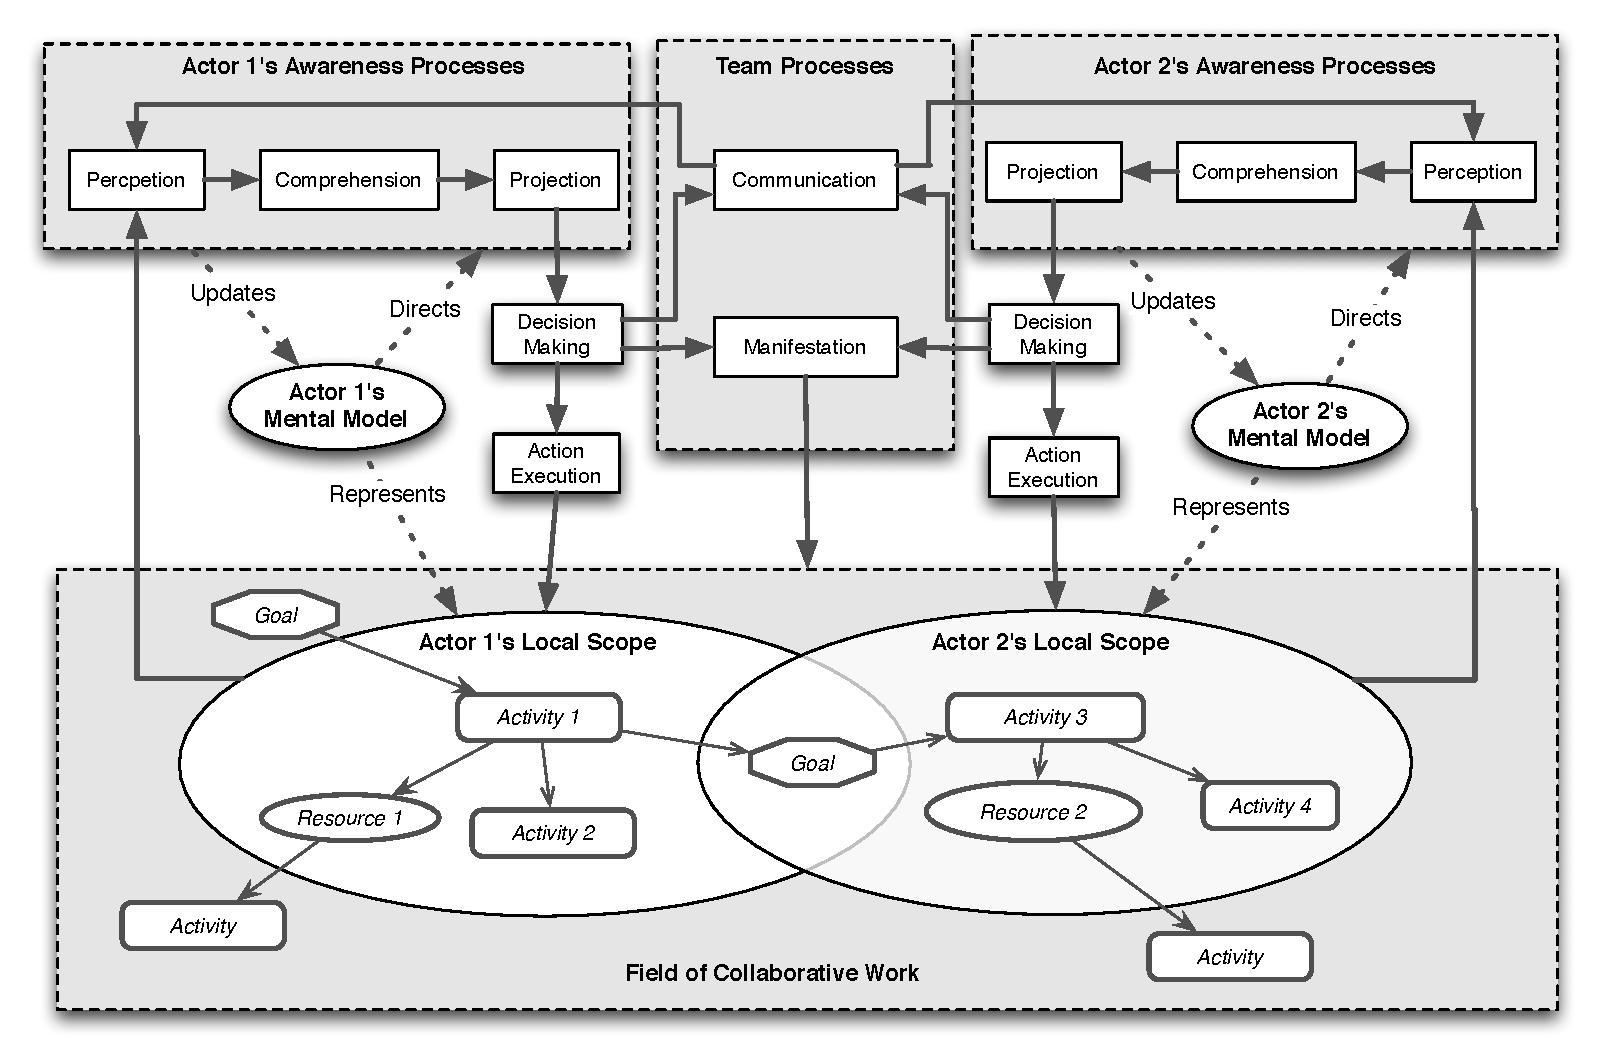
\includegraphics[width=5.5in]{conceptual_framework.pdf} 
   \caption{The Integrated Conceptual Model of Awareness}
   \label{fig:conceptual_framework}
\end{figure}

\subsection{The Field of Work} % (fold)
\label{sub:the_field_of_work}
Following the activity-directed SA model \cite{Bedny1999} and the activity awareness framework \cite{carroll2003a}, we focus on the concept of activity to structure the content of awareness, i.e. the field of collaboration work, built on top of three interrelated concepts:

\begin{enumerate}
	\item We consider \emph{activity} as the basic unit of analysis to support coordination in geo-collaboration.
	\item Due to the distributed nature of geo-collaboration, the various activities have different implications on different actors, and form their respective \emph{local scopes of work}.
	\item Activities in different local scopes of work are interdependent due to various types of \emph{dependencies} existing among them. Dependencies serve as the bridges between different local scopes of work to evaluate the implications of remote activities transcending multiple local scopes. 
	
\end{enumerate}

\subsubsection{Activity as the basic unit} % (fold)
\label{ssub:activity_basic_unit}
In our approach, we subscribe to Activity Theory to conceptualize human activities \cite{nardi1996context}. From this perspective, the basic structure of an activity can be defined as several basic elements and mutual relationships between them.

\begin{enumerate}
	\item \textbf{Actions} An action specifies a particular way of doing something. An action can be either basic or complex. A basic action can be directly executed by one or multiple actors. A complex action needs to be decomposed into subsidiary actions. When an action is specified as a sub-component of a higher action, this restricts the higher action to that particular course of doing. An action is assigned to a list of actors who are responsible to executing it.
    \item \textbf{Goals} A goal is a state of affairs in the world that the actors would like to achieve. How the condition is to be achieved is not specified, allowing alternatives to be considered. For example, a goal can only specify that a victim needs to be medically treated, but how it is achieved is not specified.
    \item \textbf{Actors} are defined as entities capable of performing actions and capable of making decisions on the performance of their actions. 
    \item \textbf{Resources} are anything that can be used in the transformation process of an action, including both material resource and resources for thinking. For example, in the case of response emergency, resources may include rescue vehicles, medical equipments, and information such as the locations of victims. 
\end{enumerate}
% paragraph relationships (end)
% subsubsection activity_basic_unit (end)

\subsubsection{Local scope of work} % (fold)
\label{ssub:local_scope_of_work}
Although various activities can be identified in a complex collaborative environment, each actor usually only engages in a small set of them. In fact, one of the fundamental motivations for team work is to decouple a complex problem into a set of smaller ones that are much easier to manage and tackle. One result of the decoupling is that the work of actors is distributed and each actor is only interested in the states of a small set of activities, resources, and conditions that are relevant to their roles, current goals and tasks. To characterize the distributed nature of team awareness, we define the local scope of work for each actor as the set of activities, resources, and conditions that have direct or potential impact on the actor’s work.

The concept of local scope of work have several characteristics of the distributed nature of emergency response activities:

\begin{enumerate}
	\item First, the local scope of work is a relative concept that changes with the actor’s current goals. Whenever an actor’s goal is changed, the local scope of work may also be changed.
	\item Second, the local scope of work may cover multiple portions of the collaborative activity as a single actor may focus on several activities at the same time. 
	\item Third, the local scopes of two actors can overlap with each other. It is common that the same activity, resource, or condition falls into the local scopes of different actors, even though it may have different impacts on these actors. Actually, these overlapping elements across multiple local scopes of work play an important role in supporting the transactive awareness process.
\end{enumerate}
% subsubsection local_scope_of_work (end)

\subsubsection{Dependencies} % (fold)
\label{ssub:dependencies}
Although activities are largely distributed and belong to local scopes of different actors, they cannot be performed without interacting with each other. Although an actor is only responsible for or interested in the activities within her/his local scope of work, the activities outside the local scope can still potentially impact her/his work through dependencies. 

Dependencies have been studied by many researchers with aspect to coordination, from organizational studies (\cite{yu1993actor,crowston1994taxonomy}), multi-agent systems (MAS) (\cite{sichman1998social,sikora1998a,sichman2002multi}), and computer-supported cooperative work (CSCW) (\cite{raposo2002coordination,cataldo2006a,de2007supporting}). Dependencies within a collaborative process can be of various forms. In general, we can summarize three types of dependency relationships that have been well recognized in the literature: temporal relationships, resource-related relationships, and goal-related relationships.

\begin{enumerate}
	\item \emph{Temporal dependencies.} The activities of the actors might be interdependent due to the constraint of ordering them in a certain order \cite{sikora1998a}. In some case, certain activities cannot be started until others are finished (the problem of sequencing) or a certain group of activities have to be performed at the same time (the problem of synchronization).
	\item \emph{Resource dependencies.} Resource dependencies can be analyzed in terms of common objects, i.e. resources, that are used by multiple actors or involved in multiple actions. An example is when two or more users simultaneously want to alter the same part of a document in a collaborative authoring system \cite{berlage1999a}. These common objects constrain how each activity is performed. Different patterns of use of the common objects by the activities will result in different kinds of dependency relationships \cite{malone1990coordination}: A \emph{fit dependency} occurs when multiple activities collectively produce the same resource. A \emph{flow dependency} arises whenever one activity produces a resource that is used by another activity. A \emph{sharing dependency} arises whenever multiple activities all use the same resource.
	\item \emph{Goal dependencies.} Goal dependencies involves the subsidiary goals that might be interdependent across various actors or their tasks \cite{sikora1998a}. A goal-related dependency reflects the fact that the depender depends on the dependee to bring about a certain state in the world. Unlike the temporal or resource-related dependencies in which the depender knows what tasks are involved in these relationships, the depender in a goal-related dependency does not care how the dependee goes about achieving the goal, i.e. the dependee is free to, and is expected to, make whatever decisions are necessary to achieve the goal \cite{yu1993actor}. A goal-related dependency is usually characterized by the structural relationship resulting from goal decomposition of the whole shared goal, i.e. task A depends on the other task B because B is a means to achieve a subsidiary goal that must be satisfied in order to perform A.
\end{enumerate}

\subsection{Awareness Processes} % (fold)
\label{sub:awareness_processes}
Built upon the field of work, a set of awareness processes can be identified to describe how the awareness is acquired and developed in a cyclical way (Figure \ref{fig:conceptual_framework}). In general, we can identify the awareness development cycles at both the individual and team levels.

\subsubsection{Individual Processes} % (fold)
\label{ssub:cognitive_processes}
At the individual level, each team member develops his/her own awareness in the similar way as described in the Neisser's perceptual cycle model \cite{neisser1976cognition}: the development of awareness starts with the perception of selective elements in the actor's local scope of work, which is then interpreted with the help of the actor's existing knowledge. The result of interpretation then help the actor to make certain decisions and perform actions, which then further update the actor's local scope of work. A important difference in our model from the original perceptual cycle model is that, instead of action directly stimulated by the acquired awareness knowledge, we emphasize the individual's planning process before the action performance, in which the individual needs to make decisions on what to do based on the interpretation of awareness information, such as whether he/she needs to change the goal, perform re-planning, or ask for help etc.

\begin{enumerate}
	\item \emph{Perception}. The process of perception is very similar to the concept in the perceptual cycle model. An actor must first be able gather perceptual information in the surrounding situation, and be able to selectively attend to those elements that are most relevant for the task at hand. The only difference is that the perception is constrained by the actor's local scope, i.e. he/she can only perceive the information about the environment, acitivities, or other objects defined in his/her local scope.
	\item \emph{Interpretation}. The process of interpretation includes generating the awareness knowledge at both the comprehension and projection levels in Endsley's three-level model \cite{Endsley1995}. The actor comprehends or understands the relevance of perceptual information in relation to their tasks and goals, and predicts likely future states in the situation.
	\item \emph{Decision Making}. The process of decision-making involves two major tasks. The first is to elaborate the actor's plan based on the interpretation. This involves decisions such as commitment to certain activity, focus switching, re-planning. The second task includes decisions about whether the actor wants to propagate the interpretation to other actors, which is important for initiating the awareness development cycle at the team level.
	\item \emph{Action}. Based on the result of decision-making process, the actor may perform some action to manipulate his/her local scope, which can lead to further changes that will start another round of perception.
\end{enumerate}

% subsubsection cognitive_processes (end)

\subsubsection{Team Processes} % (fold)
\label{ssub:interactive_processes}
\fxfatal{Elaborate on how the propagation works, three approaches: 1. explicit communication, 2. displaying via the boundary object in overlapping local scopes (need some better term: manifestation?); 3. implicit feed-through via action completion}

Beyond the individual processes of awareness development, our conceptual model allows the transactive awareness development across multiple actors in a team. The development of awareness at team level can be performed in three different trajectories

Based on the interpretation of awareness information, an actor may decide to propagate the change to other actors by indicating how the other actor's activities can be impacted by his/her interpretation. The result of propagation is then perceivable by the other actor and may initiate the other actor's individual awareness development cycle. As the other actor develops his/her individual awareness, he/she may decide to propagate his/her interpretation back to the actor or other actors in the team, or he/she may perform actions that lead to changes in other actors' local scopes. In either way, new individual cycle may be initiated and the awareness development continues at the team level.

The development of awareness at the team level is guided by the dependencies among activities and the shared activities in overlapping local scopes. The dependencies allow the actors to cascade the awareness interpretation across multiple activities. The shared activities in overlapping local scopes enable the propagation process to cross the boundary of multiple local scopes.

\subsection{An Example} % (fold)
\label{sub:an_example}
We use the motivating emergency response scenario described in Chapter 1 to show an example of the conceptual framework. 

Figure \ref{fig:field_of_work} illustrates how the different activities are distributed into different local scopes of work (represented as dotted circles) and how they are connected by the various dependency relationships. As we can see from the example, the different actors in the scenario, the victim manager, the decontamination manager, and the transportation manager, have very different roles to play, and therefore their local scopes vary significantly. However, due to the dependencies among their activities (For example, the decontamination manager relies on the transportation manager to deliver the victim to the decontamination station; the victim manager relies on the decontamination manager to perform decontamination on the victim), their local scopes are overlapped with each other.

\begin{figure}[htbp] %  figure placement: here, top, bottom, or page
   \centering
   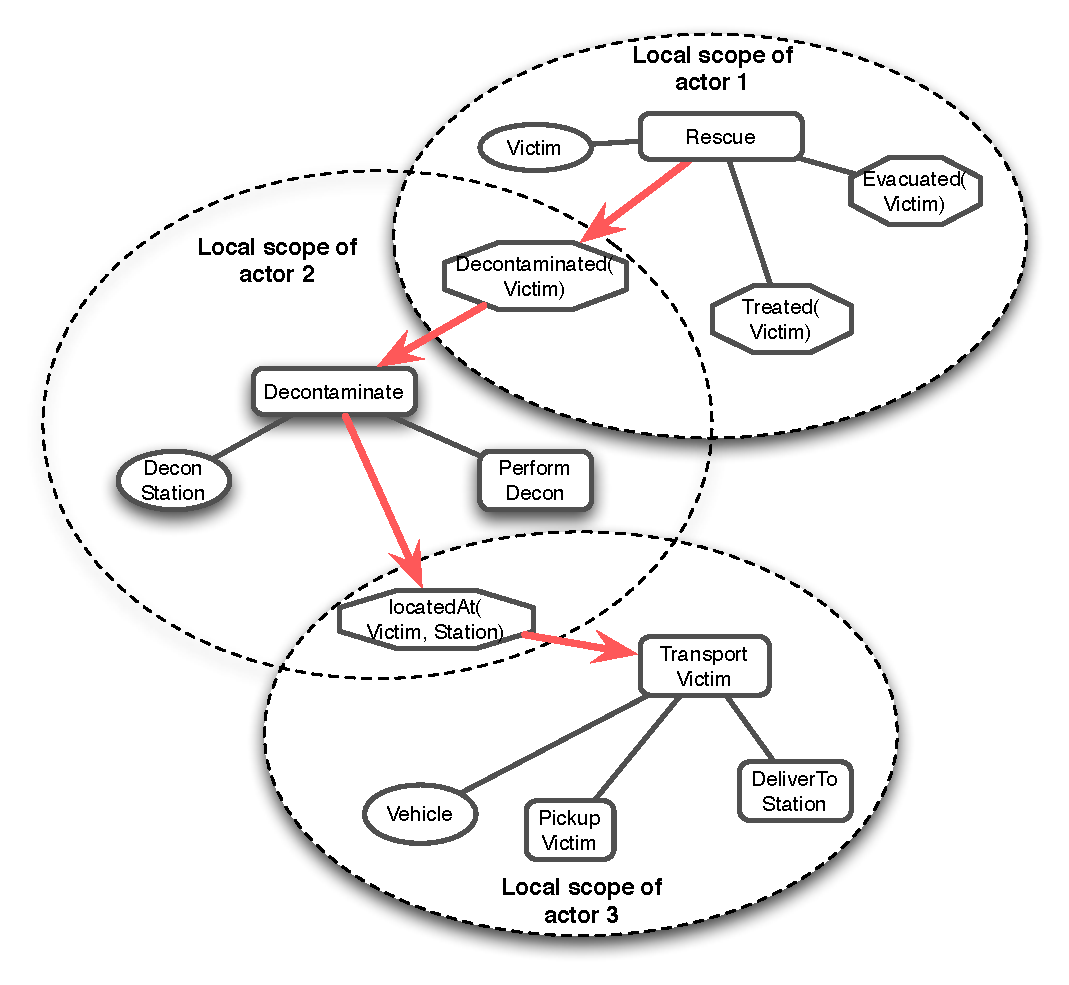
\includegraphics[width=4.5in]{field_of_work.pdf} 
   \caption{An Example: The Field of Work}
   \label{fig:field_of_work}
\end{figure}

Figure \ref{fig:awareness_process} demonstrates how the awareness processes work on top of the three constructs. In the beginning, Actor 1 perceives some unexpected event happening in the environment, and attempts to interpret it as whether and how it can impact the activities within her local scope of work. After understanding the event, she associates it with a state change of Activity 1. Furthermore, she predicts how the state change of this activity will impact other activities because of the dependencies among them. After Actor 1’s interpretation, the event is likely to impact another activity (Activity 2), and Actor 1 decides to propagate it. The propagated event falls into Actor 2’s local scope of work. Upon receiving this interpretation from Actor 1, Actor 2 first needs to understand where this event comes from by backtracking the interpretation, and evaluate how this event will impact his own line of work, which leads to a new projected state change of Activity 3. The similar process then is propagated to Actor 3’s local scope of work. In this way, the team’s awareness of the initial external event is collaborative developed as the relevant actors gradually attach their interpretations to it. 

\begin{figure}[htbp] %  figure placement: here, top, bottom, or page
   \centering
   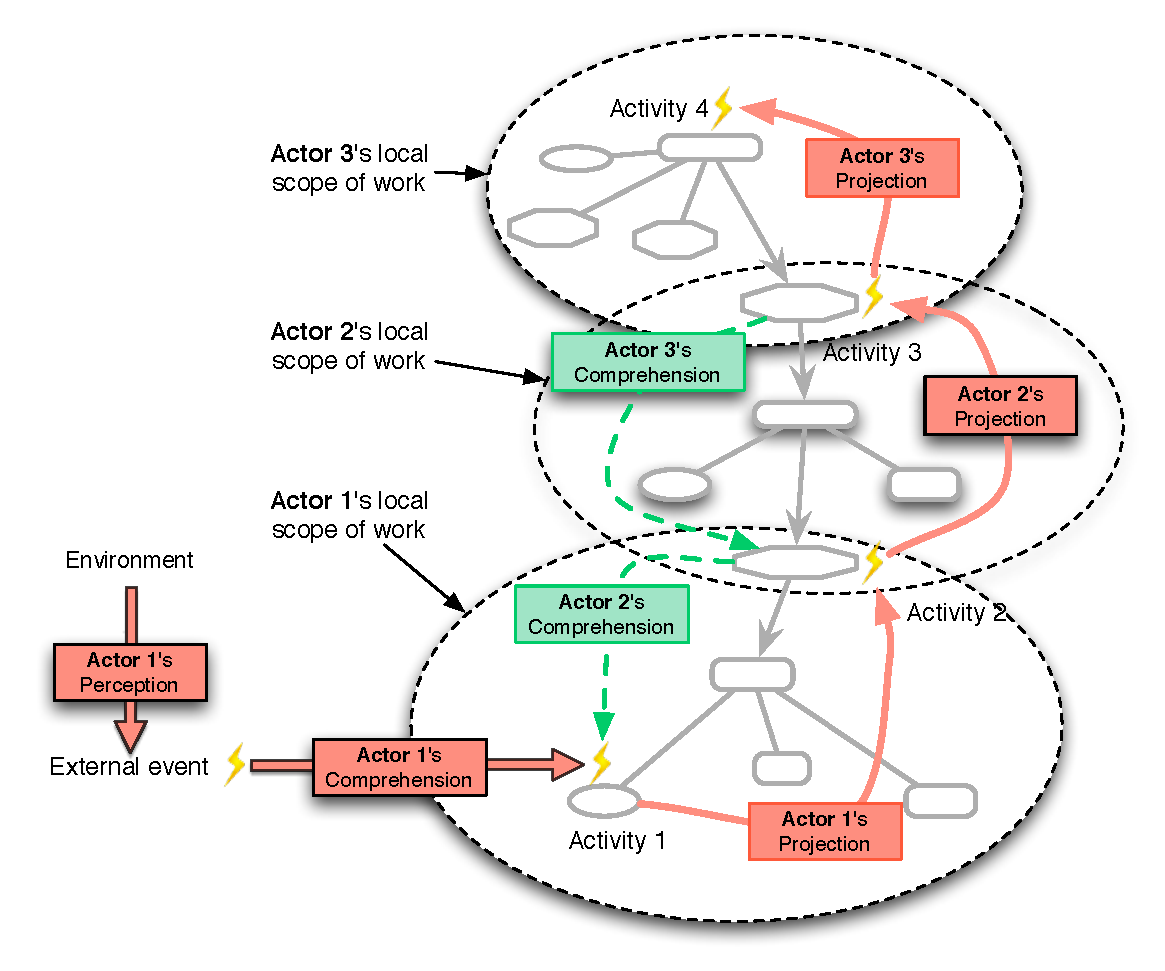
\includegraphics[width=4.5in]{awareness_process.pdf} 
   \caption{An Example: The Awareness Processes}
   \label{fig:awareness_process}
\end{figure}
% subsection an_example (end)
\subsection{Discussion} % (fold)
\label{sub:discussion}
The proposed conceptual framework shows the capabilities to satisfy the three requirements we presented in the beginning of this section.
\begin{enumerate}
	\item First, the conceptual model provides two ways to connect the individual cognitive processes and team processes. On one hand, the connection can be implicit as team members interact with the filed of work. The development of an actor's individual awareness can manipulate the field of work, which can then be perceived by other actors in their separate individual awareness processes. In addition, the actors can explicitly propagate their interpretations to other actors within their individual awareness processes.
	\item Second, the concept of local scope allows us to define how the awareness knowledge is distributed across multiple actors. The different actors often attend to different sets of activities as their local scopes. At the same time, the actors' local scopes are often overlapped due to the various dependency relationships that may occur between activities, this provides the mechanism to allow awareness transactions among multiple actors. In this way, the compatible and transactive aspects of awareness phenomena are integrated.
	\item Last, our structure of the field of work is based on the activity theory, which enables the integration of awareness and activity.  
\end{enumerate}
% subsection discussion (end)
% section discussion (end)

% chapter understanding_coordination (end)
